
\section{Portal Komposition} \label{sec:portalComposition}

\subsection{Einführung in die Architektur}
\begin{figure}
    \centering
    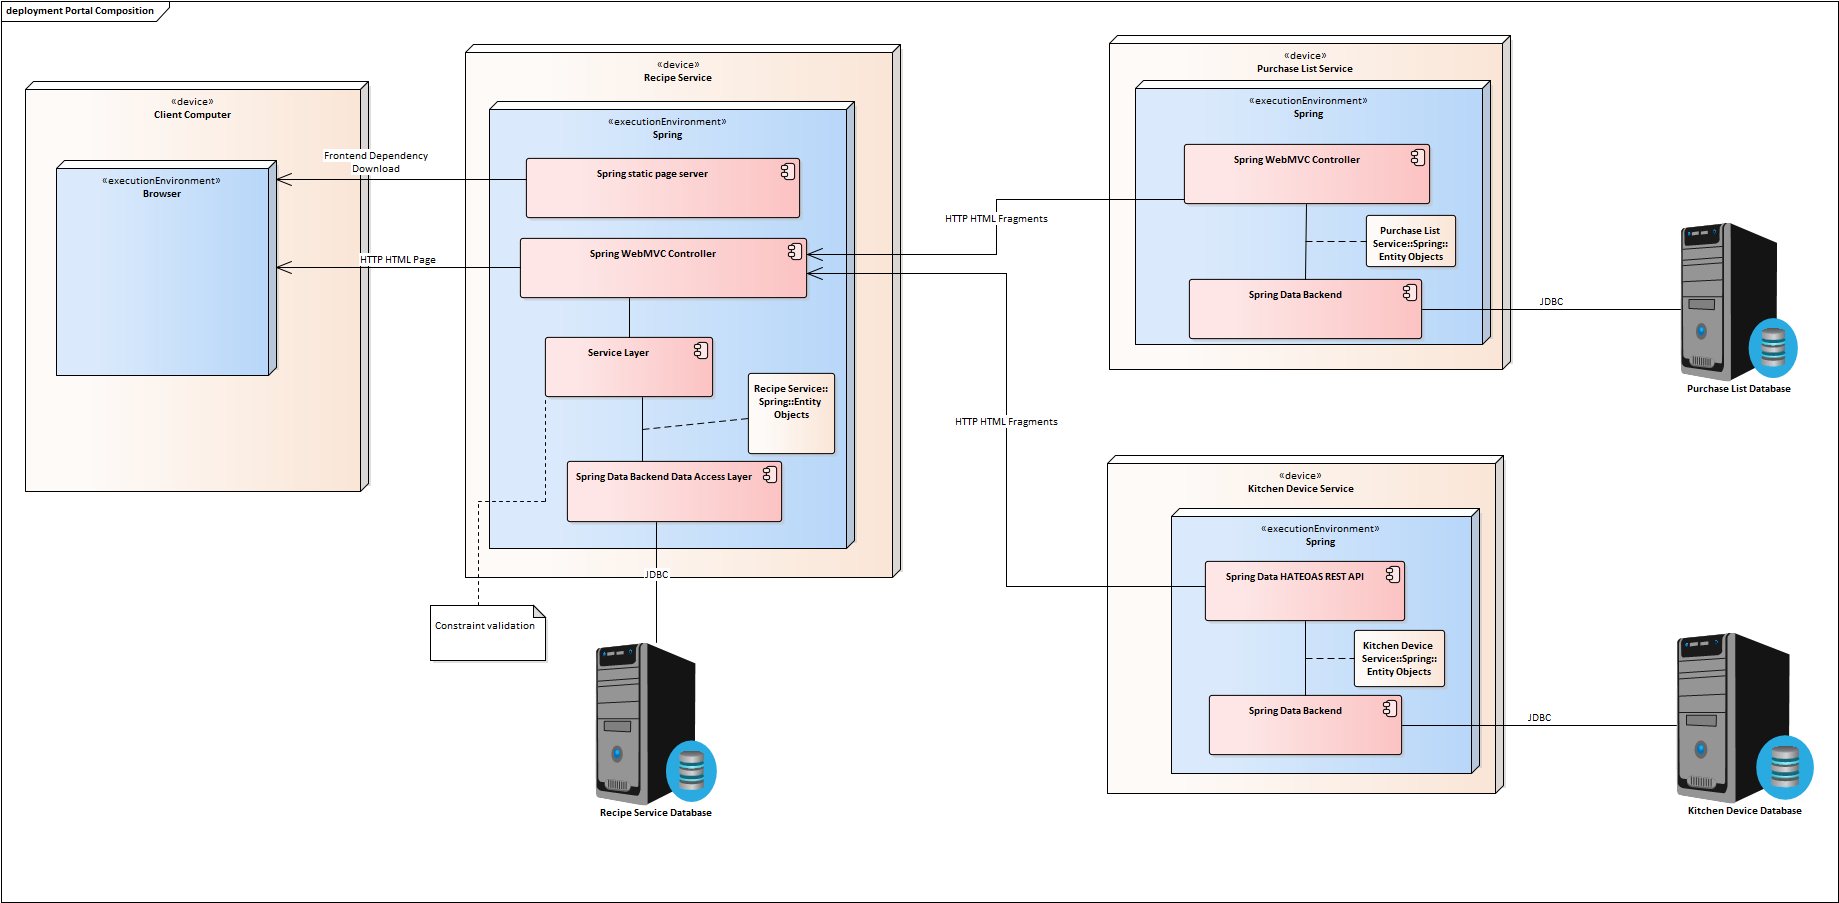
\includegraphics[width=\textwidth]{{sections/methology/assets/PortalComposition}}
    \caption{Portal Komposition}
    \label{fig:methology:portalComposition:Overview}
\end{figure}

Diese Alternative untersucht das Zusammenführen \marg{Architektur} von bestehenden Webservices in eine Portal-Architektur. Der Portal-Server führt Teilseiten von anderen Services zusammen und baut aus diesen eine gemeinsames \ac{HTML}-Dokument. Alle Links auf den Fragmenten der Hintergrundservices müssen über das Portal funktionieren. Zwischen den Services werden HTTP GET- und POST-Anfragen zu den Services versendet. Die Antworten an den Browser enthalten gültige HTML Dokumente.

Die Alternative basiert auf dem Pattern \citetitle{RichardsonFragment}\cite{RichardsonFragment} von \citeauthor{RichardsonFragment}.

Alle \marg{Implikationen} Services müssen HTML rendern können. Währenddem die Hintergrundservices die Fragmente mit den Daten rendern, muss der Portalserver die HTML-Dokumente der Seite zusammenführen in ein gemeinsames HTML-Dokument. Daraus folgt, dass alle Services einen HTML-Rendering unterstützen müssen. Der Portal-Server muss ausserdem die Integration von Drittseiten unterstützen.

Der Architekt \marg{Vorteile} erwartet die folgenden Vorteile durch die verwendete Architektur.
\begin{itemize}
    \pro Die Integration bedarf keine Änderungen an den bestehenden Services.
    \pro Die Integration kann aufgebaut werden, währendem die Anwender die bestehenden Seiten nutzen können.
\end{itemize}

Es wird erwartet, \marg{Risiken} dass die nachfolgenden Risiken bei der Implementierung der Alternative auftreten können.
\begin{itemize}
    \con Das URL-Schema des Portal-Servers muss das Schema der Hintergrundservices übernehmen.
    \con Aus dem folgt, dass es Namenskollisionen der URL-Endpunkte auf dem Portal-Server entstehen können, die schwierig zu entfernen sind.
\end{itemize}

\subsection{Implementation der Architektur}

\begin{figure}
    \centering
    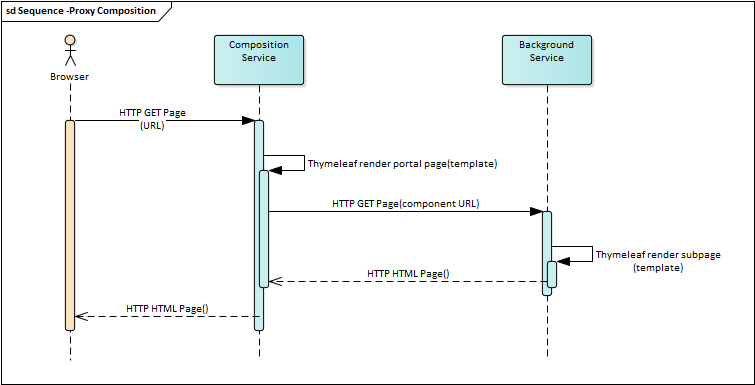
\includegraphics[width=\textwidth]{sections/methology/assets/SequencePortalComposition}
    \caption{Interaktion bei Portal Komposition}
    \label{fig:sections:methology:portalComposition:Sequence}
\end{figure}

Die Abbildung \marg{Ablauf} \ref{fig:sections:methology:portalComposition:Sequence} zeigt das Sequenz-Diagramm der Implementierung von der Portal Komposition in der Beispielanwendung. Der Browser sendet einen HTTP GET Request für die Portalseite an den Server. Dann wird der Thymeleaf Page-Renderer mit dem Page-Template aufgerufen. Durch speziellen Template-Markup im Template, das sind Befehle in der Eingabedatei vom Renderer, wird Thymeleaf im Template aufgefordert die externen Seiten nachzuladen. Beim Ladeprozess sendet der Kompositionsserver ein HTTP-Request an den Hintergrundservice. Der Service antwortet mit einem HTML-Dokument. Wenn der Kompositionsserver die Antwort enthät, extrahiert Thymeleaf einen Teil des Dokumentes und fügt ihn in die Portalseite ein. Abschliessend wird die Portalseite an den Client ausgeliefert.\footnote{https://www.thymeleaf.org/doc/articles/layouts.html\#including-with-markup-selectors}

\begin{figure}
    \centering
\begin{lstlisting}
@GetMapping("/kitchenDevice/**")
public Mono<String> kitchenDeviceService(@NotNull Model model, @NotNull HttpServletRequest request) {
    return matchPath(request).map(path -> {
        LOGGER.info("Path {} was requested", path);
        model.addAttribute(TARGET_SITE_KEY, "http://localhost:9603/controller/kitchenDevice/" + path);
        model.addAttribute(TARGET_ELEMENT_KEY, path.endsWith("edit") ? "form" : "table");
        return "portal/frameHolder";
    });
}
\end{lstlisting}
    \caption{PortalCompositionController.java, die Funktion zum Komponieren von Seiten}
    \label{fig:portalComposition:GETComposition}
\end{figure}

Der Source-Code-Block \marg{Implementierung} \ref{fig:portalComposition:GETComposition} zeigt den Code für die Portal-Komposition. Die Funktion wird für alle HTTP GET Requests auf den Kompositionspfad \texttt{/controller/kitchenDevice/} aufgerufen. Sie gibt Thymeleaf über den \texttt{model} Parameter \texttt{TARGET\_SITE\_KEY} die URL zur Ressource weiter und weisst Thymeleaf an die Seite zu rendern.

\begin{figure}
    \centering
\begin{lstlisting}
<div th:insert="${targetSite} :: ${targetElement}">...</div>
\end{lstlisting}
    \caption{Portal.html, das Page Template in welches andere Services integriert werden}
    \label{fig:portalComposition:Page}
\end{figure}
Die Thymeleaf Instruktion in Abbildung \ref{fig:portalComposition:Page} weisst Thymeleaf an ein Fragment an dieser Stelle einzusetzen. \texttt{\$\{targetSite\}} ist die URL des Dokumentes aus dem Controller und  \texttt{\$\{targetElement\}} ist der Thymeleaf Matcher \footnote{https://www.thymeleaf.org/doc/tutorials/3.0/usingthymeleaf.html\#appendix-c-markup-selector-syntax} um das zu übernehmende HTML-Element aus der Antwort des Hintergrundservices zu finden.

\subsection{Resultate aus der Programmierung der Alternative}
Die \marg{Chancen} Implementation der Portal-Komposition hat die Einfachheit der Zusammenführung von HTML-Seiten gezeigt. Das Konzept kann auch sehr generell geschrieben werden und erlaubt somit mit wenig Code die Komposition von beliebig vielen Services.

Die \marg{Risiken} Verarbeitung von POST HTTP-Requests hat sich als sehr unhandlich herausgestellt. POST-Requests müssen empfangen werden und der Body der HTTP-Message muss gelesen werden, validiert, dann neu generiert und mit WebClient neu versendet werden.

Diese Operation muss für jeden POST-Request neu programmiert werden, da sich die Body-Inhalte zwischen POST-Messages untescheiden.

Diese Implementierung von der POST HTTP Method ist sehr nahe an der Lösung der Backend-Komposition. Bei POSTs verliert die Portal-Komposition ihre wichtigste Eigenschaft, sie ist weder einfach noch generell. Sondern muss jede Message einzeln behandelt und validiert werden um Parserfehler zu verhindern.

\subsection{Diskussion der Alternative}

Die Implementierung zeigt die Machbarkeit von einer Portal Integration auf. Es wurde im Zuge dieser Arbeit einen Prototyp erstellt und getestet. 

Die Integration von HTTP POST Requests muss zurzeit individuell für jeden Request programmiert werden. Im Vergleich dazu können GET Requests mithilfe von Thymeleaf auf eine Funktion pro Service generalisiert werden.

Die \marg{Erkenntnisse} Erwartungen des Architekten (siehe \ref{sec:portalComposition}) haben sich in der Beispielapplikation gezeigt. Die Komposition konnte ohne Änderungen an den dahinterliegenden Services ausgeführt werden. Es hat sich auch gezeigt, dass bei der Integration der Applikationen Namenskollisionen auftreten können. 

In dieser Arbeit habe ich ferner gezeigt, dass eine enge Kopplung im Namensschema zwischen dem Integrationsserver und den Services entsteht. 

Der \marg{Ausblick} Architekt sieht folgende weiterführende Arbeiten:
\begin{description}
    \item[Edge Side Includes] Statt, dass die Integration in Spring Thymeleaf ausgeführt wird, kann diese auch in einem dafür optimierten Proxy ausgeführt werden. Als Beispiel seien hier Varnish\footnote{\url{https://varnish-cache.org/}} und Kong\footnote{\url{https://github.com/Kong/kong}} zu nennen.
    \item[POST Requests] Die einheitliche Behandlung von POST Requests durch den \texttt{PortalCompositionController}.
    \item[Bidirektionale Integration] Diese Beispielapplikation kann keine integrationsspezifische Parameter an die Backendservices mitgeben. Mit der Weitergabe von Identifikationsmerkmalen können Kontext spezifische Dokumente generiert werden durch die Hintergrundservices. 
\end{description}